All experiments use the simulator's own scenarios of the Agadir airspace (Moroccan upper airspace, four sectors) and
its own code; the figures are drawn from simulated situations.

\subsection{A worked example}

\Cref{fig:traj} shows the West North sector of scenario \emph{p02} at T+\exT\,s, with \exN\ aircraft on the picture and
$\Sh=\exSh\NM$. Two aircraft at FL350, \exA\ and \exB, are on routes merging at a common point; the solver predicts a
first infringement in \exTf\,s and, on a longer horizon, a closest approach of \exDmin\NM\ at \exTmin\,s: without
action they would be in trail at the same point and level. They entered the sector together, so neither has priority.

\begin{figure}[t]
\centering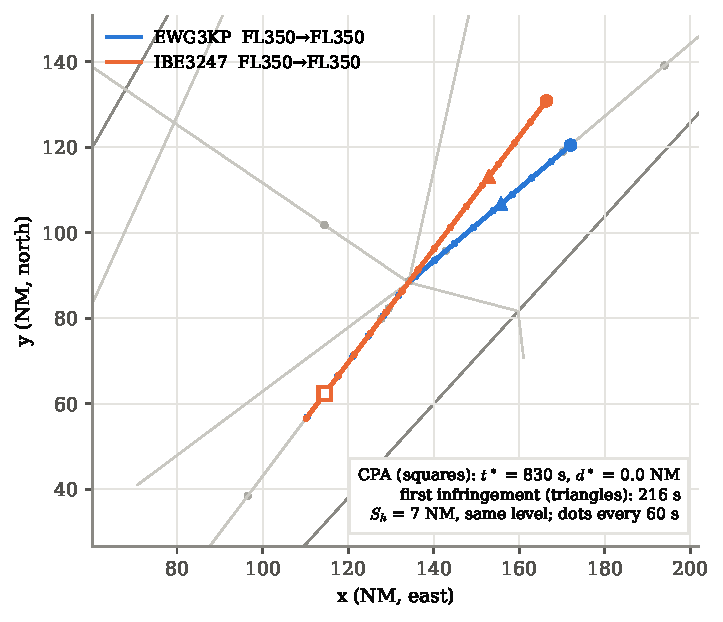
\includegraphics[width=0.72\linewidth]{figs/f1_trajectories.pdf}
\caption{Predicted piecewise-linear trajectories of a situation (grey), the conflicting pair in colour. Squares: the
closest point of approach; triangles: the first infringement of the minima, both exact (\cref{lem:cpa}).}
\label{fig:traj}
\end{figure}

\paragraph{Velocity obstacles.} \Cref{fig:vo} gives the headings of \exA\ that bring it within $\Sh$ of another aircraft
flying straight on (at its present ground speed): \exVO. Its present track \exTrk\ lies inside the obstacle of
\exB; the free arcs are \exArcs.

\begin{figure}[t]
\centering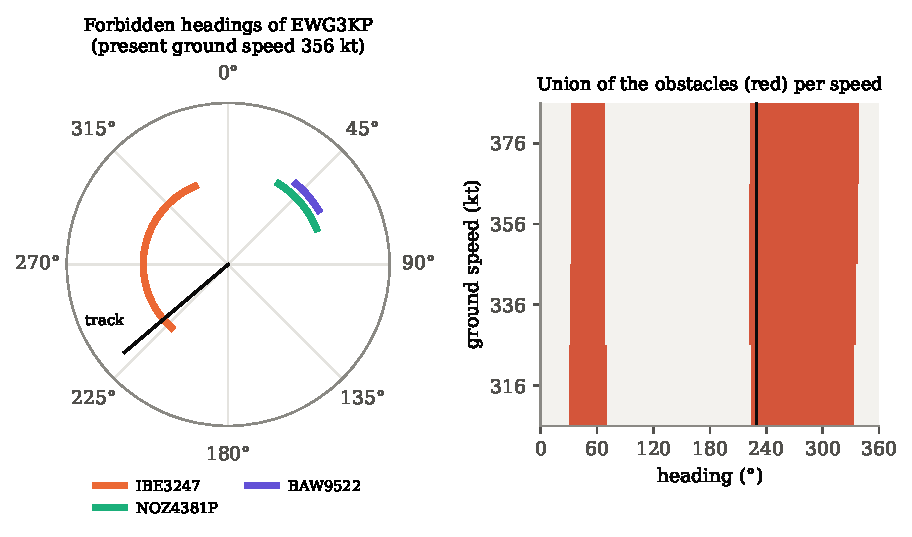
\includegraphics[width=0.95\linewidth]{figs/f3_vo.pdf}
\caption{Velocity obstacles of the aircraft to move. Left: forbidden headings per other aircraft (arcs) and the
present track. Right: their union over heading and ground speed.}
\label{fig:vo}
\end{figure}

\paragraph{Solution set.} \Cref{fig:sets} shows $\Phi$ over the plane of a delaying vector (heading change and
duration, then resume), sampled on \exGrid\ controls (\exGridMs\,ms each), and over speed alone. Speed cannot solve
this conflict: over Mach \exMachLo--\exMachHi\ the closest approach to anyone stays under \exSpeedMax\NM. The
super-level set $\{\Phi\ge\Sh+m\}$ is the region of left turns of $20^\circ$ and more; right turns bring the aircraft
towards other traffic. The solver returns \exNsol\ solutions; the optimal set is \exBest, both shortening the route
(direct before vector in the order of preference).

\begin{figure}[t]
\centering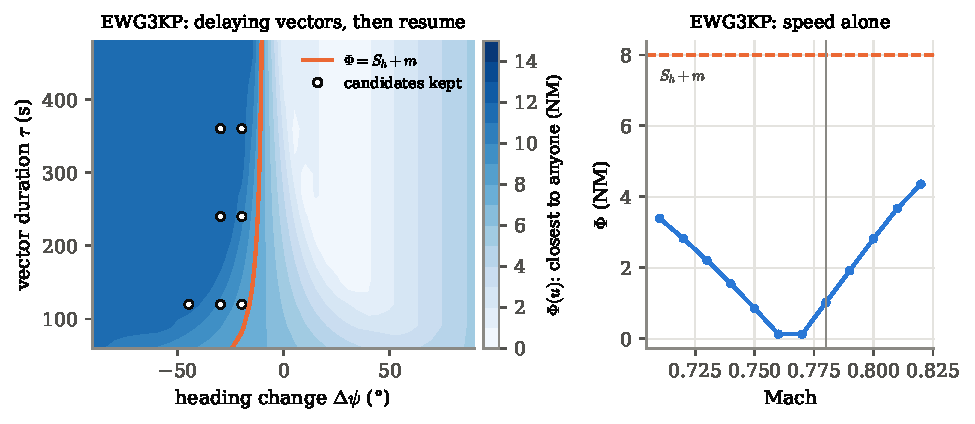
\includegraphics[width=\linewidth]{figs/f4_solutionset.pdf}
\caption{The separation function $\Phi$ of the aircraft to move. Left: over delaying vectors; the solution set is the
region beyond the orange level line $\Phi=\Sh+m$; circles: the vectors of the solver's control grid kept as
solutions. Right: over speed alone (all below $\Sh+m$).}
\label{fig:sets}
\end{figure}

\subsection{Exact CPA against sampling}

Over \cpaSits\ situations taken every two minutes in ten scenarios (aircraft not controlled), the \cpaPairs\ pairs
coming within 60\NM\ of each other were evaluated exactly and by sampling the same trajectories every $\Delta$
seconds (\cref{tab:sampling}, \cref{fig:sampling}). The error grows with $\Delta$ as \eqref{eq:sampling} predicts: up
to \cpaMaxTwenty\NM\ at 20\,s, the step of the radar's medium-term detection, and \cpaMaxSixty\NM\ at 60\,s. In
these situations no vertical window was lost and no conflict missed at any step: the main effect of sampling is the
distance it reports, which decides whether a marginal conflict is shown and whether a clearance clears it by the
margin. The windows a sampling can lose are short ones --- a climb or descent crossing another level --- which these
uncontrolled situations contain few of.

\begin{table}[t]
\centering\small
\caption{Sampled minimum minus exact minimum distance (NM) while vertically too close, over the pairs within 60\NM.
\emph{Window lost}: the sampling never sees the pair vertically too close although it is; \emph{conflicts missed}:
exact conflicts (of \cpaConf) the sampled distance does not show.}
\label{tab:sampling}
\begin{tabular}{rrrrrr}
\toprule
$\Delta$ (s) & median & 95th pct. & max & window lost & conflicts missed\\
\midrule
1 & 0.00 & 0.00 & 0.04 & 0 & 0 \\
5 & 0.00 & 0.01 & 0.21 & 0 & 0 \\
10 & 0.00 & 0.03 & 0.35 & 0 & 0 \\
20 & 0.00 & 0.06 & 0.70 & 0 & 0 \\
30 & 0.00 & 0.29 & 1.95 & 0 & 0 \\
60 & 0.00 & 1.02 & 4.02 & 0 & 0 \\
\bottomrule

\end{tabular}
\end{table}

\begin{figure}[t]
\centering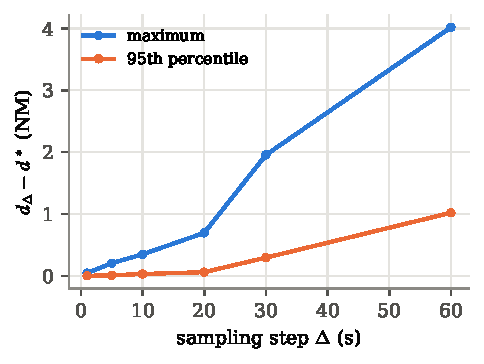
\includegraphics[width=0.48\linewidth]{figs/f2_sampling.pdf}
\caption{Error of a sampled minimum distance against the exact CPA.}
\label{fig:sampling}
\end{figure}

\subsection{Reachability}

\Cref{fig:hj} shows slices of the zero level set of $V$ for $\Sh=5\NM$ and equal speeds. Without turning, any
aircraft in the band ahead whose straight path crosses the disk is a conflict; with turns at standard rate, the set
from which the conflict cannot be avoided within five minutes shrinks to a region a few miles ahead of the moved
aircraft, longest head-on.

To validate the table and the frame used to look it up, \hjN\ relative states within 25\NM\ were drawn at random and
the encounter simulated in the plane: the moved aircraft turns left or right at $3^\circ$/s for 0 to 300\,s and then
flies straight, the other flies straight, and the best of these strategies gives a lower bound of the true value.
The sign of $V$ agrees with the simulation in \hjAgree\% of the states (\cref{fig:hjval}). Near the boundary the
table is slightly optimistic (mean \hjMeanNear\NM, median \hjMedNear\NM, part of which is the simulation's restricted
strategies). With the threshold $\mu=\MUval\NM$, no state the simulation finds unavoidable (\hjUnav) is declared
avoidable by turning, at the price of \hjCons\ avoidable states declared unavoidable --- the safe side.

\begin{remark}
The validation found an error in an earlier version: the relative state was expressed with $y$ to the left of the
track while the tables' dynamics, with clockwise track angles, hold for $y$ to the right --- the lookup was of the
mirror-image encounter. On the \hjMirN\ states where the two frames differ by more than 1.5\NM, the mean error is
\hjMirOk\NM\ in the right frame and \hjMirBad\NM\ in the mirrored one.
\end{remark}

\begin{figure}[t]
\centering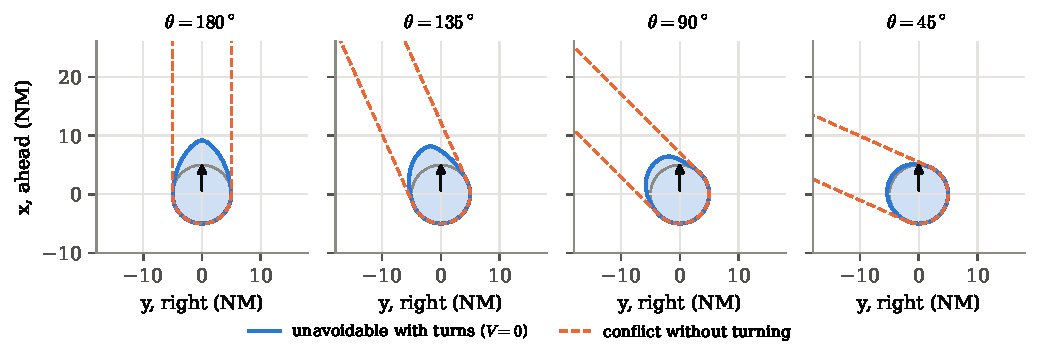
\includegraphics[width=\linewidth]{figs/f5_hj_slices.pdf}
\caption{Slices $\theta=\mathrm{const}$ of the reachability tables ($\Sh=5\NM$, $v_2=v_1=450$\,kt, $T=300$\,s). The
moved aircraft is at the origin heading up (arrow); the other is at $(y,x)$ with track difference $\theta$. Blue: the
states from which no turn avoids the loss; dashed: the conflicts of straight flight; grey: the target disk.}
\label{fig:hj}
\end{figure}

\begin{figure}[t]
\centering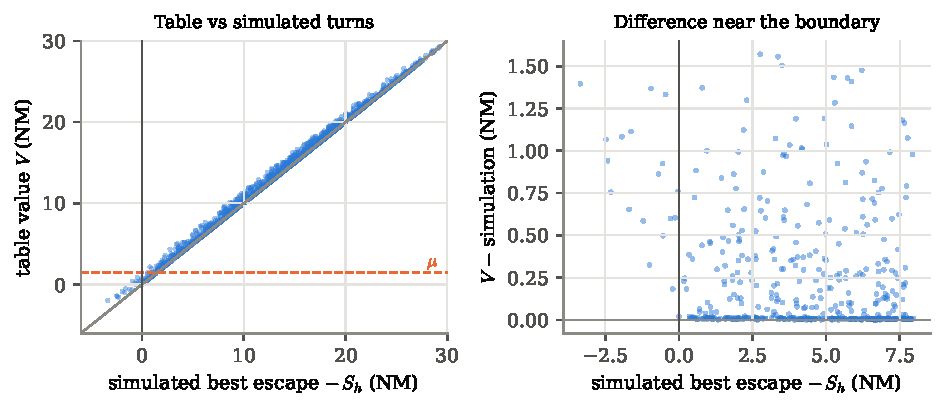
\includegraphics[width=\linewidth]{figs/f6_hj_validation.pdf}
\caption{Validation of the reachability table against simulated turns: the table value against the best simulated
escape (left), and their difference near the boundary (right).}
\label{fig:hjval}
\end{figure}

\subsection{The solver on frozen situations}

On the same situations (\stN\ aircraft each), predicting all trajectories and computing the conflict matrix took a
median of \stMatMed\,ms (at most \stMatMax\,ms); the cost grows with the number of pairs (\cref{fig:stats}, left).
As no one controls these situations, the same encounter appears in several of them until it
becomes a loss: the solver met \stDistinct\ distinct encounters in \stScn\ scenarios, \stConf\ times in all:
\stFut\ times ahead of the encounter, and \stCur\ times already in a loss of separation (no clearance can make $\Phi\ge\Sh+m$ there: the distance is already below the minimum, and the
observation instead gives the levels that separate soonest). It found solutions for \stSolved\ of the \stFut\ future
conflicts (\stSolvedPct\%); the best solution's kind was: \stKinds. The \stUnsolved\ others were close (median time to
infringement \stUnsolvedTf\,s), where only a combination or action on the other traffic remains. A complete solve,
including the rollouts, took a median of \stSolveMed\,s per situation with conflicts (at most \stSolveMax\,s) on a
shared two-core machine. Each rollout of a ten-minute horizon costs about \ROLLval\,s. For the \stConfirmed\
solutions confirmed by rollout, \cref{fig:stats} (right) compares the predicted margin over the minimum with the margin
in the simulation. The simulation is mostly the more favourable --- the prediction keeps every aircraft on its
route while the pilots of the copy also resume, turn and level off as they fly --- and in \stBelowPred\ cases it is
more than half a mile less favourable, at worst by \stWorstGap\NM\ --- more than the margin $m$ covers, which is
why the best solutions are confirmed before they are proposed.

\begin{figure}[t]
\centering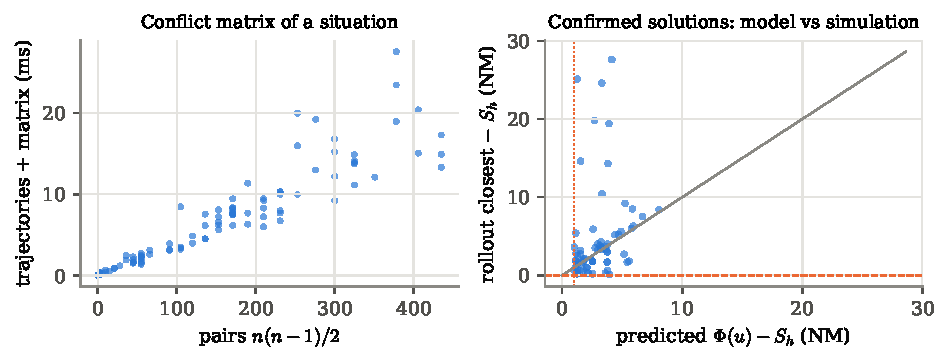
\includegraphics[width=\linewidth]{figs/f7_solver_stats.pdf}
\caption{Left: cost of the trajectory prediction and conflict matrix of a situation against the number of pairs.
Right: for the solutions confirmed by rollout, the margin over $\Sh$ predicted against the margin in the
simulation (dotted: the margin $m$ required of a solution; dashed: the minimum).}
\label{fig:stats}
\end{figure}

\subsection{Closed loop: the solver as a controller}

Finally the solver controlled \clN\ scenarios for 20 simulated minutes each through the AI lab, against the
built-in baseline controller, which assumes, transfers and answers requests the same way but resolves conflicts with
its own rules (speed, then a probed heading, then a level). Both were scored by the lab's evaluation (100 minus
penalties: 25 per loss of separation, 10 per infringement of an active area, track miles, late assumes and
transfers\dots). \Cref{tab:runs} gives the results. Mean score: solver \clSolverMean\ (\clSolverLoss\ losses in
all), baseline \clBaselineMean\ (\clBaselineLoss\ losses). Graded against the solver's solution sets, the baseline's
conflict decisions were: \clBaseGrades\ (the baseline acts on conflicts under eight minutes only, hence the many
conflicts left alone at a given decision).

Neither controller handles the activation of restricted areas (scenario s10) or the non-RVSM aircraft of p05, which
cost both the same penalties; the difference between them is in the losses of separation. The closed loop was also
how two weaknesses of an earlier version of the trajectory model were found. In p06 the solver controller approved a
pilot's request for descent that the radar's probe, with a nominal 2000\,ft/min, found clear; the aircraft, high on
its profile, descended at idle with speedbrakes, at almost twice that, through the level of an aircraft 5\NM\ away,
and was mid-turn after a point. The prediction now flies turns in progress (\cref{sec:traj}) and checks level changes
at the bounds of the rates (\cref{prop:rates}); requests are approved only when both the probe and the solver's check
find them clear.

\begin{table}[t]
\centering\small
\caption{Twenty-minute runs. Score (0--100), losses of separation, clearances given (speed / heading or direct /
level) and the smallest separation in a loss (NM).}
\label{tab:runs}
\setlength{\tabcolsep}{4pt}
\begin{tabular}{l rrcr rrcr}
\toprule
& \multicolumn{4}{c}{Baseline} & \multicolumn{4}{c}{Solver}\\
\cmidrule(lr){2-5}\cmidrule(lr){6-9}
Scenario & score & loss & spd/lat/lvl & min & score & loss & spd/lat/lvl & min\\
\midrule
c01\_cta\_moderate\_wx & 100.0 & 0 & 0/1/0 & -- & 100.0 & 0 & 0/0/0 & -- \\
p01\_ws\_two\_merges & 74.4 & 1 & 0/4/0 & 6.5 & 100.0 & 0 & 0/3/0 & -- \\
p02\_wn\_merges\_and\_climbs & 100.0 & 0 & 0/3/0 & -- & 100.0 & 0 & 9/1/0 & -- \\
p05\_ws\_storms\_arrivals & 95.0 & 0 & 0/0/0 & -- & 95.0 & 0 & 0/0/0 & -- \\
p06\_wn\_capacity\_sequencing & 74.0 & 1 & 0/8/0 & 6.6 & 100.0 & 0 & 0/2/0 & -- \\
s01\_basic\_crossing & 100.0 & 0 & 0/1/0 & -- & 100.0 & 0 & 3/1/0 & -- \\
s02\_climb\_request\_into\_crossing & 100.0 & 0 & 0/0/0 & -- & 100.0 & 0 & 0/0/0 & -- \\
s03\_descent\_through\_opposite & 100.0 & 0 & 0/0/0 & -- & 100.0 & 0 & 0/0/0 & -- \\
s05\_slowdown\_on\_converging\_exit & 100.0 & 0 & 1/1/0 & -- & 100.0 & 0 & 1/0/0 & -- \\
s06\_speed\_up\_into\_crossing & 100.0 & 0 & 3/1/0 & -- & 100.0 & 0 & 1/1/0 & -- \\
s08\_simultaneous\_level\_requests & 100.0 & 0 & 0/0/0 & -- & 100.0 & 0 & 0/0/0 & -- \\
s10\_busy\_mixed & 70.0 & 0 & 7/7/0 & -- & 70.0 & 0 & 1/7/0 & -- \\
\midrule
Mean & 92.8 & 2 & & & 97.1 & 0 & & \\
\bottomrule

\end{tabular}
\end{table}
